
\section{\label{sec:Tutorial-Subduction}Tutorial for Slip on a Subduction
Zone}

PyLith features discussed in this tutorial:
\begin{itemize}
\item Static solution
\item Quasi-static solution
\item CUBIT mesh generation

\begin{itemize}
\item Nonplanar geometry
\item Variable mesh resolution
\item APREPRO programming language
\end{itemize}
\item Linear triangular cells
\item HDF5 output
\item Dirichlet displacement and velocity boundary conditions
\item ZeroDispDB spatial database
\item SimpleDB spatial database
\item UniformDB spatial database
\item Multiple materials
\item Nonlinear solver
\item Plane strain linearly elastic material
\item Plane Maxwell linear viscoelastic material
\item Prescribed slip

\begin{itemize}
\item Static fault rupture
\item Multiple faults
\item Spatially variable coseismic slip
\item Spatially variable aseismic creep
\end{itemize}
\item Afterslip via fault friction

\begin{itemize}
\item Static fault rupture
\item Static friction
\end{itemize}
\end{itemize}
All of the files necessary to run the examples are contained in the
directory \texttt{examples/2d/subduction.}


\subsection{Overview}

This tutorial examines quasi-static interseismic and coseismic deformation
in 2D for a subduction zone (see Figure \ref{fig:tutorial:subduction:overview}).
It is based on the 2011 M9.0 Tohoku earthquake off the east coast
of Japan. Figure \ref{fig:tutorial:subduction:steps} shows the three
steps of increasing complexity. Step 1 focuses on the coseismic slip,
Step 2 focuses on interseismic deformation, and Step 3 combines the
two into a pseudo-earthquake cycle deformation simulation. Step 4
focuses on using the change in tractions from Step 1 to construct
a simulation with afterslip controlled by frictional sliding.

\begin{figure}
\begin{centering}
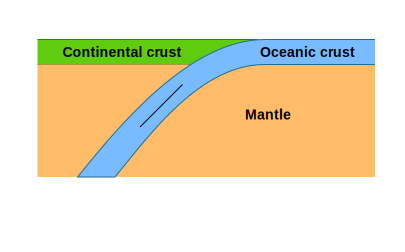
\includegraphics{tutorials/subduction/figs/cartoon_general}
\par\end{centering}

\caption{Cartoon of subduction zone example.\label{fig:tutorial:subduction:overview}}
\end{figure}


\begin{figure}
\begin{centering}
\begin{tabular}{ccc}
Step 1 & Step 2 & Step 3\tabularnewline
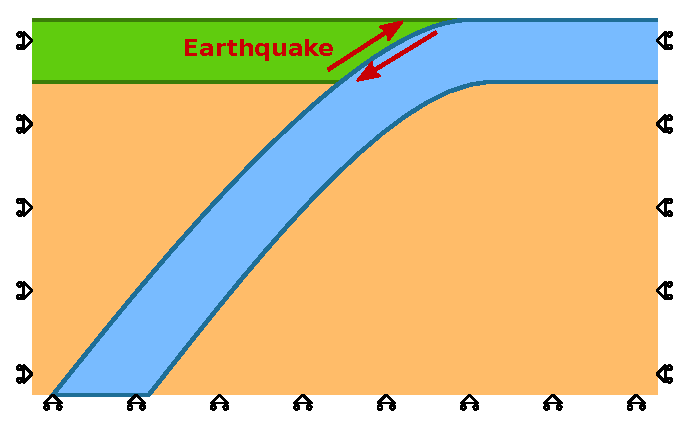
\includegraphics[width=2in]{tutorials/subduction/figs/step01} & 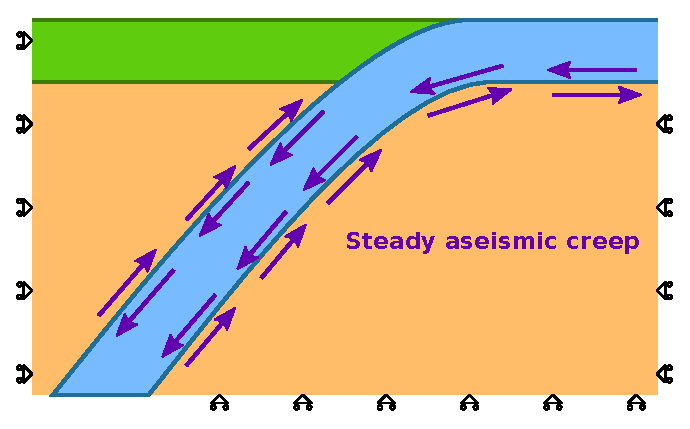
\includegraphics[width=2in]{tutorials/subduction/figs/step02} & 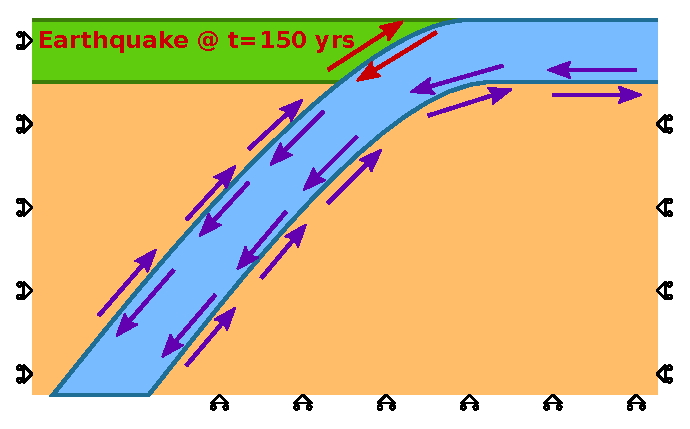
\includegraphics[width=2in]{tutorials/subduction/figs/step03}\tabularnewline
\end{tabular}
\par\end{centering}

\caption{Diagram of fault slip and boundary conditions for each step in the
subduction zone tutorial.\label{fig:tutorial:subduction:steps}}
\end{figure}



\subsection{Mesh Description}

We construct the mesh in CUBIT by constructing the geometry, prescribing
the discretization, running the mesher, and then grouping cells and
vertices for boundary conditions and materials. We use the APREPRO
programming language within the journal files to enable use of units
and to set variables for values used many times. An appendix in the
CUBIT documentation discusses the features available with APREPRO
in CUBIT. The CUBIT commands are in three separate journal files.
The main driver is in the journal file \texttt{mesh\_tri3.jou}. It
calls the journal file \texttt{geometry.jou} to construct the geometry
and \texttt{createbc.jou} to set up the groups associated with boundary
conditions and materials. The journal files are documented and describe
the various steps outlined below.
\begin{enumerate}
\item Create the geometry defining the domain.

\begin{enumerate}
\item Create points.
\item Connect points into spline curves.
\item Split curves to separate them into sections bounding surfaces. 
\item Connect curves into surfaces.
\item Stitch surfaces together.
\end{enumerate}
\item Define meshing scheme and cell size variation.

\begin{enumerate}
\item Define cell size along curves near fault.
\item Increase cell size away from fault at a geometric rate (bias).
\end{enumerate}
\item Generate mesh.
\item Create blocks for materials and nodesets for boundary conditions.
\item Export mesh.
\end{enumerate}
\begin{figure}
\begin{centering}
\includegraphics[width=4.5in]{tutorials/subduction/figs/subduction_tri3}
\par\end{centering}

\caption{Variable resolution finite-element mesh with triangular cells. The
nominal cell size increases at a geometric rate of 1.2 away from the
region of coseismic slip.\label{fig:tutorial:subduction:mesh}}
\end{figure}



\subsection{Common Information}

As in the examples discussed in previous sections of these tutorials,
we place parameters common to the three steps in the \texttt{pylithapp.cfg}
file so that we do not have to duplicate them for each step. The settings
contained in \texttt{pylithapp.cfg} for this problem consist of:
\begin{description}
\item [{pylithapp.journal.info}] Settings that control the verbosity of
the output written to stdout for the different components.
\item [{pylithapp.mesh\_generator}] Settings that control mesh importing,
such as the importer type, the filename, and the spatial dimension
of the mesh.
\item [{pylithapp.timedependent}] Settings that control the problem, such
as the total time, time-step size, and spatial dimension.
\item [{pylithapp.timedependent.materials}] Settings that control the material
type, specify which material IDs are to be associated with a particular
material type, and give the name of the spatial database containing
the physical properties for the material. The quadrature information
is also given.
\item [{pylithapp.problem.formulation.output}] Settings related output
of the solution over the domain and subdomain (ground surface).
\item [{pylithapp.timedependent.materials.\textit{MATERIAL}.output}] Settings
related to output of the state variables for material \textit{MATERIAL}.
\item [{pylithapp.petsc}] PETSc settings to use for the problem, such as
the preconditioner type.
\end{description}
The physical properties for each material are specified in spatial
database files. For example, the elastic properties for the continental
crust are in \texttt{mat\_concrust.spatialdb}. The provided spatial
database files all use just a single point to specify uniform physical
properties within each material. A good exercise is to alter the spatial
database files with the physical properties to match PREM.


\subsection{Step 1: Coseismic Slip Simulation}

The first example problem is earthquake rupture involving coseismic
slip along the interface between the subducting slab and the continental
crust and uppermost portion of the mantle below the continental crust.
The spatial variation of slip comes from a cross-section of Gavin
Hayes' finite-source model \url{earthquake.usgs.gov/earthquakes/eqinthenews/2011/usc0001xgp/finite_fault.php}.
On the lateral and bottom boundaries of the domain, we fix the degrees
of freedom perpendicular to the boundary as shown in Figure \ref{fig:tutorial:subduction:steps}.
Parameter settings that augment those in \texttt{pylithapp.cfg} are
contained in the file \texttt{step01.cfg}. These settings are:
\begin{description}
\item [{pylithapp.timedependent.formulation.time\_step}] Adjust the total
simulation time to 0 years (static simulation).
\item [{pylithapp.timedependent}] Specifies the array of boundary conditions.
\item [{pylithapp.timedependent.bc.\textit{BOUNDARY}}] Defines the settings
for boundary \textit{BOUNDARY}, including which degrees of freedom
are being constrained (x or y), the label (defined in\texttt{ mesh\_tri3.exo})
corresponding to the nodeset in CUBIT, and a label to the boundary
condition used in any error messages.
\item [{pylithapp.timedependent.interfaces.fault}] Specify the coseismic
slip along the interface between the oceanic crust and continental
crust with a small amount of slip penetrating into the upper mantle.
\item [{pylithapp.problem.formulation.output.domain}] Gives the base filenames
for HDF5 output (for example, \texttt{step01.h5}).
\end{description}
We run this example by typing
\begin{lyxcode}
pylith~step01.cfg
\end{lyxcode}
The problem will produce twelve pairs of HDF5/Xdmf files. The HDF5
files contain the data and the Xdmf files contain the metadata required
by ParaView and Visit (and possibly other visualization tools that
use Xdmf files) to access the mesh and data sets in the HDF5 files.
The files include the solution over the domain and ground surface
(two pairs of files), physical properties, stress, and strain within
each material (eight pairs of files), and fault parameters, slip,
and traction (two pairs of files). 

Figure \ref{fig:tutorial:subduction:step01}, which was created using
ParaView, displays the magnitude of the displacement field with the
deformation exaggerated by a factor of 1000. 

\noindent \begin{center}
\begin{figure}
\begin{centering}
\includegraphics[width=4.5in]{tutorials/subduction/figs/step01_soln}
\par\end{centering}

\caption{Solution for Step 1. The colors indicate the magnitude of the displacement,
and the deformation is exaggerated by a factor of 1000. \label{fig:tutorial:subduction:step01}}
\end{figure}

\par\end{center}


\subsection{Step 2: Interseismic Deformation Simulation}

In this example we simulate the interseismic deformation associated
with the oceanic crust subducting beneath the continental crust and
into the mantle. We prescribe steady aseismic slip of 8 cm/yr along
the interfaces between the oceanic crust and mantle with the interface
between the oceanic crust and continental crust locked as shown in
Figure \ref{fig:tutorial:subduction:steps}. We adjust the Dirichlet
boundary conditions on the lateral edges and bottom of the domain
by pinning only the portions of the boundaries in the mantle and continental
crust (i.e., not part of the oceanic crust). Parameter settings that
augment those in \texttt{pylithapp.cfg} are contained in the file
\texttt{step02.cfg}. These settings include:
\begin{description}
\item [{pylithapp.timedependent.formulation.time\_step}] Adjust the total
simulation time to 100 years.
\item [{pylithapp.timedependent}] Specifies the array of boundary conditions.
\item [{pylithapp.timedependent.bc.\textit{BOUNDARY}}] Defines the settings
for boundary \textit{BOUNDARY}, including which degrees of freedom
are being constrained (x or y), the label (defined in\texttt{ mesh\_tri3.exo})
corresponding to the nodeset in CUBIT, and a label to the boundary
condition used in any error messages.
\item [{pylithapp.timedependent.interfaces}] Specify the steady aseismic
slip as a constant slip rate on the fault surfaces. 
\item [{pylithapp.problem.formulation.output.domain}] Gives the base filename
for HDF5 output (for example, \texttt{step02.h5}).
\end{description}
We run this example by typing
\begin{lyxcode}
pylith~step02.cfg
\end{lyxcode}
The simulation will produce pairs of HDF5/Xdmf files with separate
files for each material and fault interface. Figure \ref{fig:tutorial:subduction:step02},
which was created using ParaView, displays the magnitude of the displacement
field with the deformation exaggerated by a factor of 1000. Using
the animation features within ParaView or Visit you can illustrate
how the continental crust near the trench subsides during the interseismic
deformation. 

\noindent \begin{center}
\begin{figure}
\begin{centering}
\includegraphics[width=4.5in]{tutorials/subduction/figs/step02_soln}
\par\end{centering}

\caption{Solution for Step 2 at 100 years. The colors indicate the magnitude
of the displacement, and the deformation is exaggerated by a factor
of 1000.\label{fig:tutorial:subduction:step02}}
\end{figure}

\par\end{center}


\subsection{Step 3: Pseudo-Earthquake Cycle Model}

This simulation combines 300 years of interseismic deformation from
Step 2 with the coseismic deformation from Step 1 applied at 150 years
to create a simple model of the earthquake cycle. Parameter settings
that augment those in \texttt{pylithapp.cfg} are contained in the
file \texttt{step03.cfg}. These settings include:
\begin{description}
\item [{pylithapp.timedependent.formulation.time\_step}] Adjust the total
simulation time to 300 years.
\item [{pylithapp.timedependent}] Specifies the array of boundary conditions.
\item [{pylithapp.timedependent.bc.\textit{BOUNDARY}}] The Dirichlet boundary
conditions match those in Step 2.
\item [{pylithapp.timedependent.interfaces}] On the interface between the
subducting oceanic crust and the mantle, we prescribe the same steady,
aseismic slip as that in Step 2. On the interface along the top of
the subducting oceanic crust and the continental crust and mantle
we create two earthquake ruptures, The first rupture applies the coseismic
slip form Step 1 at 150 years, while the second rupture prescribes
the same steady, aseismic slip as in Step 2.
\item [{pylithapp.problem.formulation.output.domain}] Gives the base filename
for HDF5 output (for example, \texttt{step03.h5}).
\end{description}
We run this example by typing
\begin{lyxcode}
pylith~step03.cfg
\end{lyxcode}
The simulation will produce pairs of HDF5/Xdmf files with separate
files for each material and fault interface. Figure \ref{fig:tutorial:subduction:step03},
which was created using ParaView, displays the magnitude of the displacement
field with the deformation exaggerated by a factor of 1000. Using
the animation features within ParaView or Visit you can illustrate
how the continental crust near the trench rebounds during the earthquake
after subsiding during the interseismic deformation. 

\noindent \begin{center}
\begin{figure}
\begin{centering}
\includegraphics[width=4.5in]{tutorials/subduction/figs/step03_soln}
\par\end{centering}

\caption{Solution for Step 3 at 150 years (immediately following the earthquake
rupture). The colors indicate the magnitude of the displacement, and
the deformation is exaggerated by a factor of 1000.\label{fig:tutorial:subduction:step03}}
\end{figure}

\par\end{center}


\subsection{Step 4: Frictional Afterslip Simulation}

This simulation demonstrates how to combine the change in tractions
associated with coseismic slip with a background stress field to compute
afterslip controlled by static friction. The Python script \texttt{afterslip\_tractions.py}
will create a spatial database file with initial tractions based on
the change in tractions from Step 1 and a background stress field.
The background stress field is simply normal tractions consistent
with the overburden (lithostatic load) for a uniform half-space and
shear tractions consistent with a coefficient of friction of 0.6.
The \texttt{afterslip\_tractions.}~\linebreak{}
\texttt{spatialdb} file is provided, so you do not need to run the
Python script \texttt{afterslip\_tractions.py}; however, you can do
so by typing
\begin{lyxcode}
python~afterslip\_tractions.py
\end{lyxcode}
We provide 2.0 MPa of strength excess associated with the background
stress field by using a cohesion of 2.0 MPa in the static friction
model. Slip will occur in regions where the coseismic slip increased
the shear tractions by more than 2.0 MPa. On the lateral and bottom
boundaries of the domain, we fix the degrees of freedom perpendicular
to the boundary as shown in Figure \ref{fig:tutorial:subduction:steps}.
Parameter settings that augment those in \texttt{pylithapp.cfg} are
contained in the file \texttt{step04.cfg}. These settings are:
\begin{description}
\item [{pylithapp.timedependent.formulation.time\_step}] Adjust the total
simulation time to 0 years (static simulation).
\item [{pylithapp.timedependent}] Selects the nonlinear solver and specifies
the array of boundary conditions.
\item [{pylithapp.timedependent.bc.\textit{BOUNDARY}}] Defines the settings
for boundary \textit{BOUNDARY}, including which degrees of freedom
are being constrained (x or y), the label (defined in\texttt{ mesh\_tri3.exo})
corresponding to the nodeset in CUBIT, and a label to the boundary
condition used in any error messages.
\item [{pylithapp.timedependent.interfaces.fault}] Specify a fault with
a fault constitutive model (static friction) and initial fault tractions. 
\item [{pylithapp.problem.formulation.output.domain}] Gives the base filenames
for HDF5 output (for example, \texttt{step04.h5}).
\end{description}
We run this example by typing
\begin{lyxcode}
pylith~step04.cfg
\end{lyxcode}
The problem will produce twelve pairs of HDF5/Xdmf files. The HDF5
files contain the data and the Xdmf files contain the metadata required
by ParaView and Visit (and possibly other visualization tools that
use Xdmf files) to access the mesh and data sets in the HDF5 files.
The files include the solution over the domain and ground surface
(two pairs of files), physical properties, stress, and strain within
each material (eight pairs of files), and fault parameters, slip,
and traction (two pairs of files). 

Figure \ref{fig:tutorial:subduction:step04}, which was created using
ParaView, displays the magnitude of the displacement field with the
original configuration. Slip occurs down-dip from the coseismic slip
as well as in three areas with sharp gradients in slip, including
the trench. The location of the afterslip can be shifted by changing
the spatial variation of the coseismic slip and background stress
field.

\noindent \begin{center}
\begin{figure}
\begin{centering}
\includegraphics[width=4.5in]{tutorials/subduction/figs/step01_soln}
\par\end{centering}

\caption{Solution for Step 4. The colors indicate the magnitude of the displacement.
\label{fig:tutorial:subduction:step04}}
\end{figure}

\par\end{center}


\subsection{Suggested Variations}

The list below includes some suggested modifications to the problem
that will allow you to become more familiar with PyLith while examining
some interesting physics.
\begin{itemize}
\item Change the resolution of the mesh by editing the \texttt{mesh\_tri3.jou}
journal file. Change the resolution and bias factor.
\item Add depth dependent viscosity to the mantle and crust. This requires
using the linear Maxwell plane strain bulk constitutive model in the
crust as well and creating spatial databases that include viscosity
for the crust. Specifying a depth dependent variation in the parameters
will require adding points, updating num-locs accordingly, and changing
data-dim to 1.
\item Modify the spatial database files for the material properties to use
depth-dependent elastic properties based on PREM (Dziewonski and Anderson,
1981, 10.1016/0031-9201(81)90046-7). See \url{geophysics.ou.edu/solid_earth/prem.html}
for a simple table of values. Add points, update num-locs accordingly,
and change data-dim to 1.
\item Modify the CUBIT journal files to use quad4 cells rather than tri3
cells. This requires using the pave mesh scheme.
\item Create a simulation with multiple earthquake cycles by lengthening
the duration of the simulation and adding additional earthquake ruptures.
See \texttt{examples/3d/hex8/step06.cfg} for an example with multiple
earthquake ruptures. Examine spinup towards a steady-state solution.\end{itemize}

